\section{Complemento}

\subsection{Redes de adaptación L}

La red L es una red de adaptación cuya funcion es hacer que haya máxima transferencia de potencia de una fuente hacia un carga. Esta compuesta por dos elementos reactivos puestos
en forma de L entre la resisitencia de la fuente y la carga. Las cuatro configuraciones posibles y sus ecuaciones de diseño son:

% imagen del primer circuito

\begin{figure}[H]
    \centering
    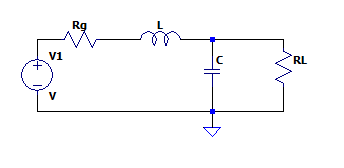
\includegraphics[width=0.5\textwidth]{imagenes/redesL1.png}
    \caption{Red L en configuración 1}
    \label{fig:redL1}
\end{figure}

Donde $R_L$ es mayor que $R_s$. Este es un filtro pasa bajos.

% ecuacion de Q L y C

%raiz de RL/Rs-1
\begin{equation}
    Q = \sqrt{\frac{R_L}{R_s}-1}
\end{equation}

% L igual a Q por Rs dividido 2 pi f
\begin{equation}
    L = Q \cdot \frac{R_s}{2 \pi f}
\end{equation}

% C igual a Q dividido por 2 pi  f por RL
\begin{equation}
    C = \frac{Q}{2 \pi f R_L}
\end{equation}


% imagen del segundo circuito

\begin{figure}[H]
    \centering
    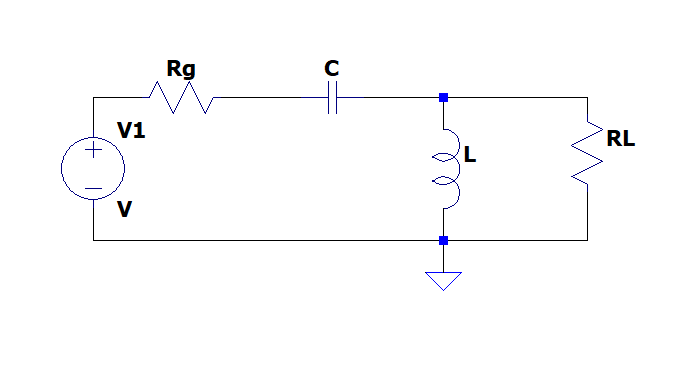
\includegraphics[width=0.5\textwidth]{imagenes/redesL2.png}
    \caption{Red L en configuración 2}
    \label{fig:redL2}
\end{figure}

Donde $R_L$ es mayor que $R_s$. Ademas con este circuito producimos un desacople de continua y es un filtro pasa altos.


% ecuacion de Q L y C

%raiz de RL/Rs-1
\begin{equation}
    Q = \sqrt{\frac{R_L}{R_s}-1}
\end{equation}

% L igual a RL dividido por 2 pi f Q
\begin{equation}
    L = \frac{R_L}{2 \pi f Q}
\end{equation}

% C igual a 1 dividido por 2 pi f Q Rs
\begin{equation}
    C = \frac{1}{2 \pi f Q R_s}
\end{equation}


% imagen del tercer circuito

\begin{figure}[H]
    \centering
    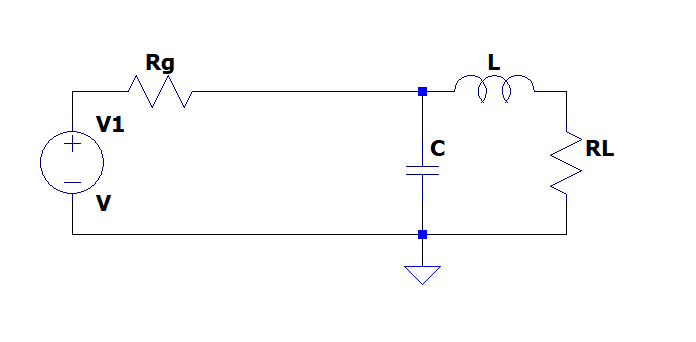
\includegraphics[width=0.5\textwidth]{imagenes/redesL3.png}
    \caption{Red L en configuración 3}
    \label{fig:redL3}
\end{figure}

Donde $R_L$ es menor que $R_s$. Es un filtro pasa bajos.

% ecuacion de Q L y C

%raiz de Rs/RL-1
\begin{equation}
    Q = \sqrt{\frac{R_s}{R_L}-1}
\end{equation}

% L igual a Q por RL dividido por 2 pi f
\begin{equation}
    L = Q \cdot \frac{R_L}{2 \pi f}
\end{equation}

% C igual a Q por Rl dividido por 2 pi f Rs
\begin{equation}
    C = \frac{Q}{2 \pi f R_s}
\end{equation}


% imagen del cuarto circuito

\begin{figure}[H]
    \centering
    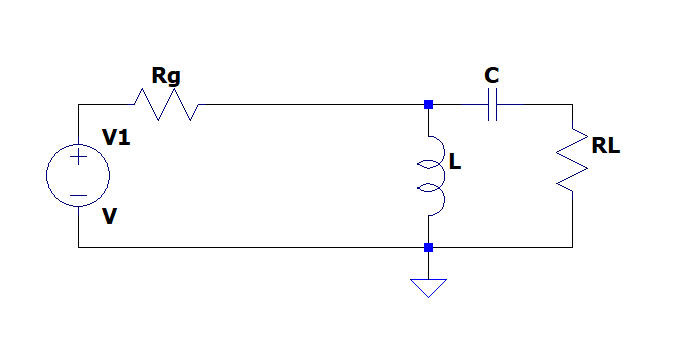
\includegraphics[width=0.5\textwidth]{imagenes/redesL4.png}
    \caption{Red L en configuración 4}
    \label{fig:redL4}
\end{figure}

Donde $R_L$ es menor que $R_s$. Ademas con este circuito producimos un desacople de continua y es un filtro pasa altos.

% ecuacion de Q L y C

%raiz de Rs/RL-1
\begin{equation}
    Q = \sqrt{\frac{R_s}{R_L}-1}
\end{equation}

% L igual a Rs dividido por 2 pi f Q
\begin{equation}
    L = \frac{R_s}{2 \pi f Q}
\end{equation}

% C igual a 1 dividido por 2 pi f Q RL
\begin{equation}
    C = \frac{1}{2 \pi f Q R_L}
\end{equation}


En todas las configuraciones la frecuencia central de resosnancia es:

\begin{equation}
    f_0 = \frac{1}{2 \pi \sqrt{L \cdot C}}
\end{equation}

Esta red es la configuracion mas sencilla pero tiene la desventaja de que el factor de calidad no es ajustable. Las aplicaciones mas comunes de las redes de 
adaptación L son:

\begin{itemize}
    \item En sistemas de audio para adaptar impedancias entre etapas de amplificación.
    \item En sistemas de comunicación para adaptar etapas de transmisión y recepción.
    \item Filtros pasa bajos y pasa altos.
\end{itemize}


